\chapter{Experimental Framework}

\MyQuote{What we observe is not nature itself, but nature exposed to our method of
questioning.}{Werner Heisenberg}

In the previous chapter, the key features of QCD - today's theory of strong
interaction - were introduced. The predictions of QCD are tested at particle
accelerators persistently and there is the whole army of theoretical physicists
awaiting new discovery unexplainable in the terms of QCD.
Unfortunately for them, there is no such measurement which would not be in
agreement with QCD predictions up to date but the Large Hadron Collider can
change this very soon.

In this chapter, the QCD will be raised from the theoretical description of the
previous chapter, to the practical implementation on Large Hadron Collider,
which will be described with emphasize on the ATALS detector. The all important
concept of particle physics of hadron colliders - jet - will be introduced in
this chapter.

\section{The Large Hadron Collider and The ATLAS Detector}

\subsection{The Large Hadron Collider}

The Large Hadron Collider (LHC) \cite{LHC, LHCPastPresentFuture} is a charged
particle accelerator located on the border of France and Switzerland, near
Geneva. Built using the areas of the Large Electron-Positron collider, the main
accelerator ring, of a 27 km circumference, is located around 100 m below the
surface. There are four main experiments located around the ring: A Large Ion
Collider Experiment (ALICE), A Toroidal LHC ApparatuS (ATLAS), Compact Muon
Solenoid (CMS) and Large Hadron Collider beauty (LHCb). The complete accelerator
and detector system is shown at Figure \ref{fig:LHC}.

\begin{figure}[t]
  \centering
  \includegraphics[width=0.8\textwidth]{Chapter2/LHC.jpg}
  \caption{This diagram shows the locations of the four main experiments (ALICE,
    ATLAS, CMS and LHCb) that take place at the LHC. Located between 50 m and
    150 m underground, huge caverns have been excavated to house the giant
    detectors. The Super Proton Synchotron (SPS), the final link in the
    pre-acceleration chain, and its connection tunnels to the LHC are also
    shown.  Figure from \cite{CERN:ATLASexperimentPictureswiki}  }
  \label{fig:LHC}
\end{figure}

LHC started to operate on November 23, 2009 and soon thereafter (March 30, 2010)
the proton-proton collisions achieved the center-of-mass energy $\sqrt{s} = 7
\TeV$, which is halve of the design energy of the machine. On April 5, 2012, the
machine started its successful $\sqrt{s} = 8 \TeV$ run.

Next to the proton-proton collisions first heavy-ion Pb-Pb collisions took place
in 2010 at a center of mass energy per pair of colliding nucleons $\sqrt{s} =
2.76 \TeV$. Proton-Pb collisions at $\sqrt{s} = 5.02 \TeV$ occurring on LHC
during 3 weeks of 2013 successfully demonstrated LHC capability to provide
asymmetric collisions.  

The first running period of the LHC, RunI, was very successful and resulted in
important discoveries including Higgs boson on July 4, 2012
\cite{HiggsDiscovery}.  The accelerator complex has been upgraded including its
experiments for two years and it is expected, the Run II will start in summer
2015 \cite{LHCFuture, LHCFutureLuminosigy}. In Run II the center-of-mass energy of proton-proton
collisions will be raised up to $\sqrt{s} = 13 \TeV$ and beam crossing time will
be reduced from the current $50\,\text{ns}$ to $25\,\text{ns}$. Integrated
luminosity in RunII will cross $100\,\text{fb}^{-1}$.

\subsection{The ATLAS Detector}

The ATLAS detector \cite{ATLAS} is a general-purpose detector surrounding one of
the interaction points of the LHC and with $\sim 100$ million of individual
electronic channels it is the most complicated instrument ever created having
one simple task: Record charged particle collisions up to the center-of-mass
energy per pair of colliding nucleons $\rts = 14 \TeV$. A detector overview is
shown in Figure~\ref{fig:ATLASfull}, where the main sub-detector systems can be
seen: the inner detector, used to reconstruct charged-particle tracks, the
electromagnetic calorimeters, the hadronic calorimeters, and the muon
spectrometer. 

\begin{figure}[p]
  \centering
  \begin{subfigure}[b]{0.9\textwidth}
    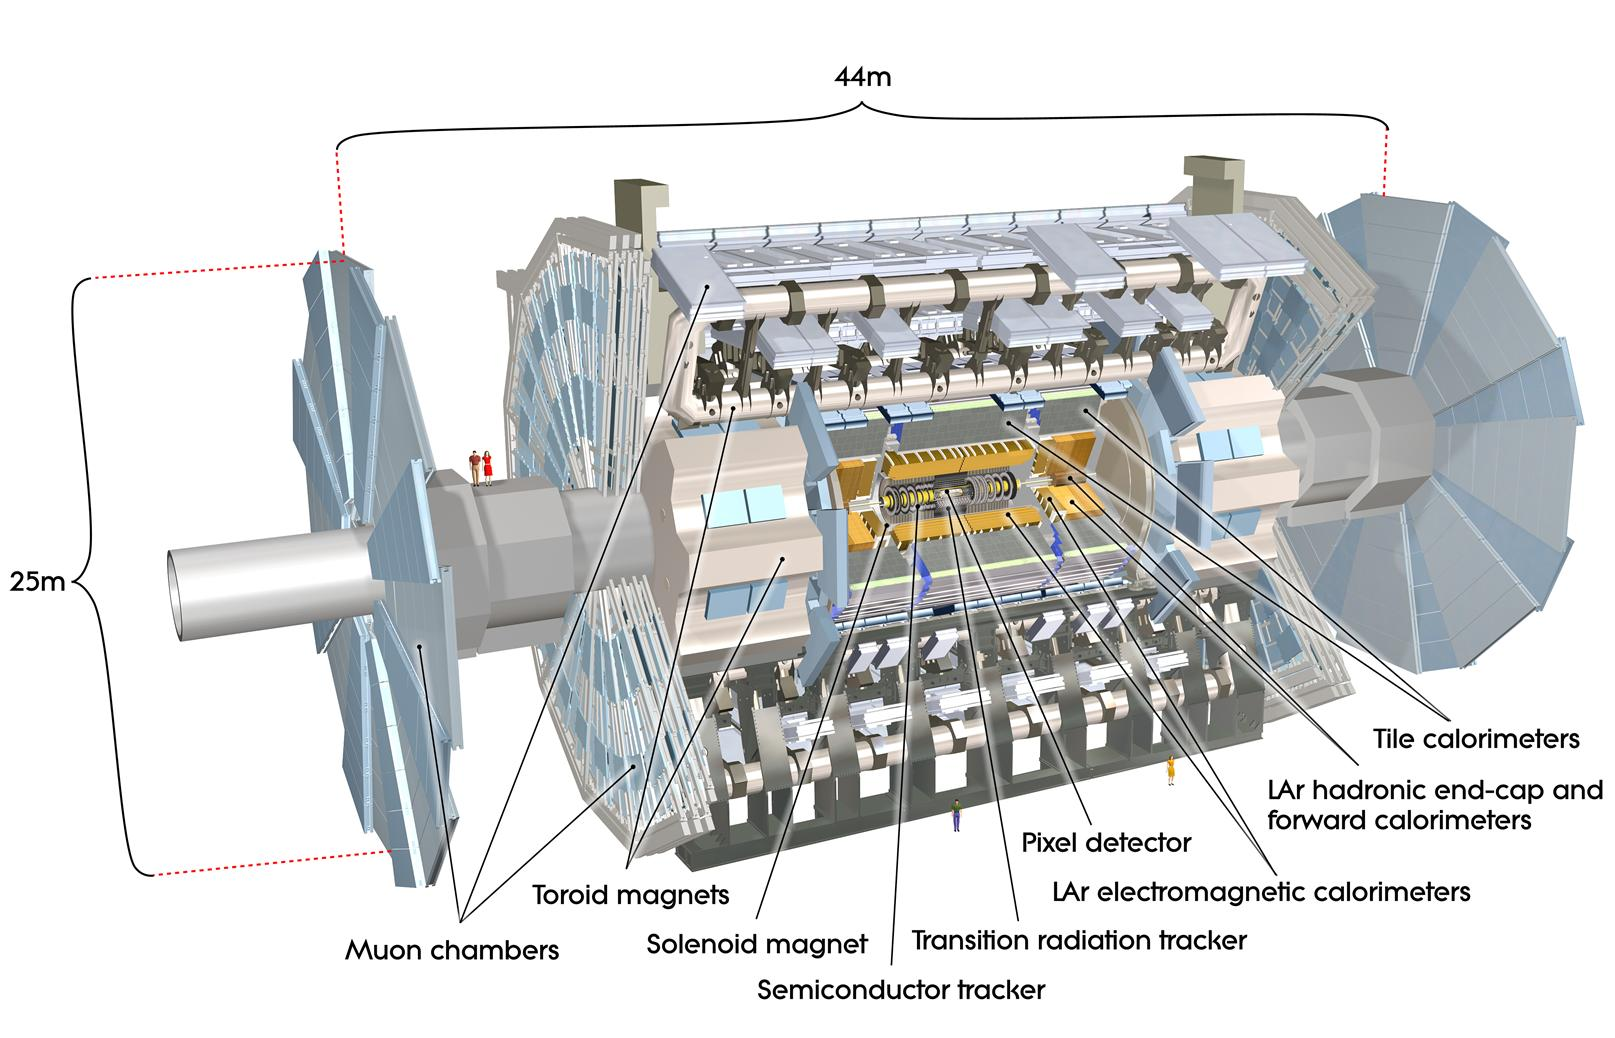
\includegraphics[width=\textwidth]{Chapter2/ATLAS.png}
    \caption{ATLAS detector}
    \label{fig:ATLASfull}
  \end{subfigure}
  ~
  \begin{subfigure}[b]{0.9\textwidth}
    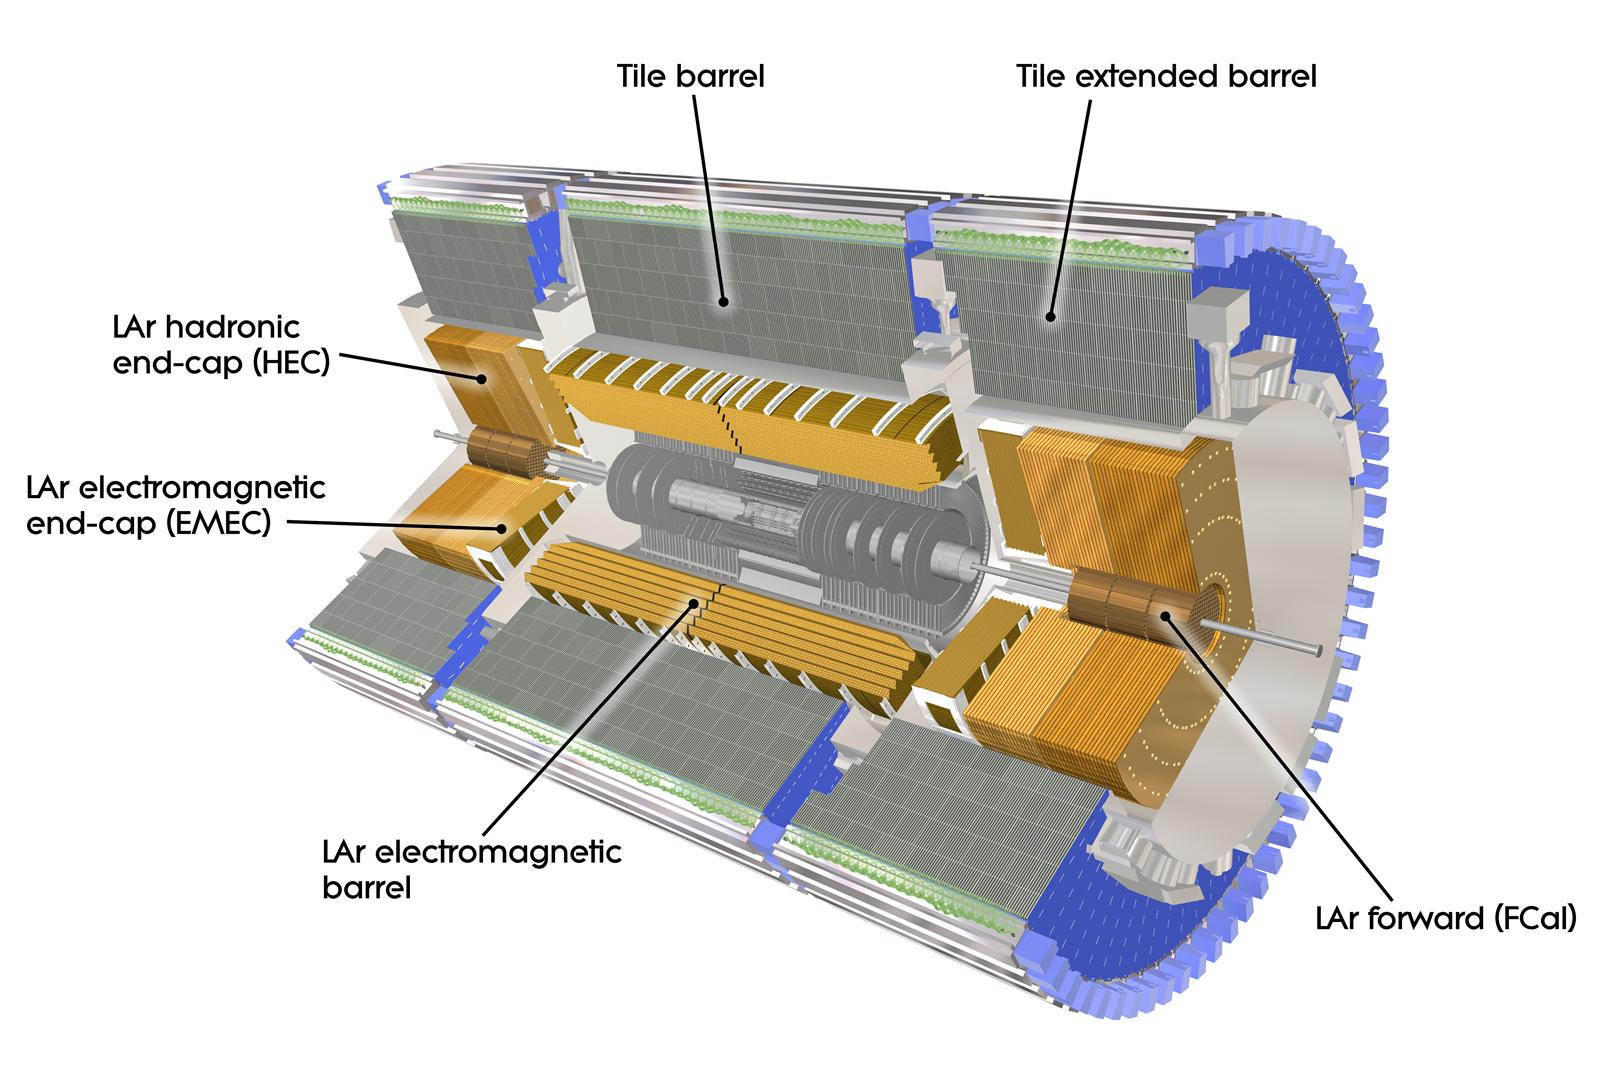
\includegraphics[width=\textwidth]{Chapter2/ATLASinner.jpeg}
    \caption{Inner detector and calorimeter systems}
    \label{fig:ATLASinner}
  \end{subfigure}
  \caption{(a) an overview of the ATLAS detector 
           (b) detail on the inner detector and the calorimeters - the dominant
           sub-detector systems used in this thesis. Figures from
           \cite{CERNbook}.}
  \label{fig:ATLAS}
\end{figure}

ATLAS uses a right-handed coordinate system with its origin at the interaction
point in the center of the detector and the $z$ axis along the beam pipe. The
$x$ axis points from the interaction point to the center of the LHC ring, and
the $y$ axis points upward. Cylindrical coordinates $(r, \phi)$ are used in the
transverse plane, $\phi$ being the azimuthal angle around the beam pipe. Instead
of polar angle $\theta$ pseudorapidity $\eta$ is used throughout this thesis. For
event selection the rapidity $y$ plays an important role. In following
definitions of pseudorapidity $\eta$ and rapidity $y$, $E$ stands for the total
energy and $p$ for size of total momentum: 
\begin{eqnarray}
  \eta &= & - \frac{1}{2} \ln \left( \frac{p+p_z}{p-p_z} \right) = - \ln \left[
  \tan \left( \frac{\theta}{2} \right) \right], \\ y &= &- \frac{1}{2} \ln
  \left( \frac{E+p_z}{E-p_z} \right).	
\end{eqnarray}
The transverse momentum $\pt$ presents the component of momentum perpendicular
to the beam line.  

The main detector system relevant to this thesis is the ATLAS calorimeter,
which is emphasized in Figure~\ref{fig:ATLASinner}. The calorimeter is divided
into sub-detectors, providing overall coverage up to $|\eta| < 4.9$. The
electromagnetic calorimeter, covering region $|\eta| < 3.2$, is a
high-granularity sampling detector in which the active medium is liquid argon
(LAr) interspaced with layers of lead absorber. The hadronic calorimeters are
divided into three sections: a tile scintillator/steel calorimeter is used in
both the barrel ($|\eta| < 1.0$) and extended barrel cylinders ($0.8 < |\eta| <
1.7$) while the hadronic endcap ($1.5 < |\eta| < 3.2$) consists of LAr/copper
calorimeter modules. The forward calorimeter measures both electromagnetic and
hadronic energy in the range $3.2 < |\eta| < 4.9$ using LAr/copper and
LAr/tungsten modules. 

\section{Hadron Collision at LHC}

In this section the phenomenological description of proton-proton collisions
will be presented following picture in Figure \ref{fig:HardProcess} and
Reference about Monte Carlo event generators \cite{PDG}.

\begin{figure}[t]
  \centering
  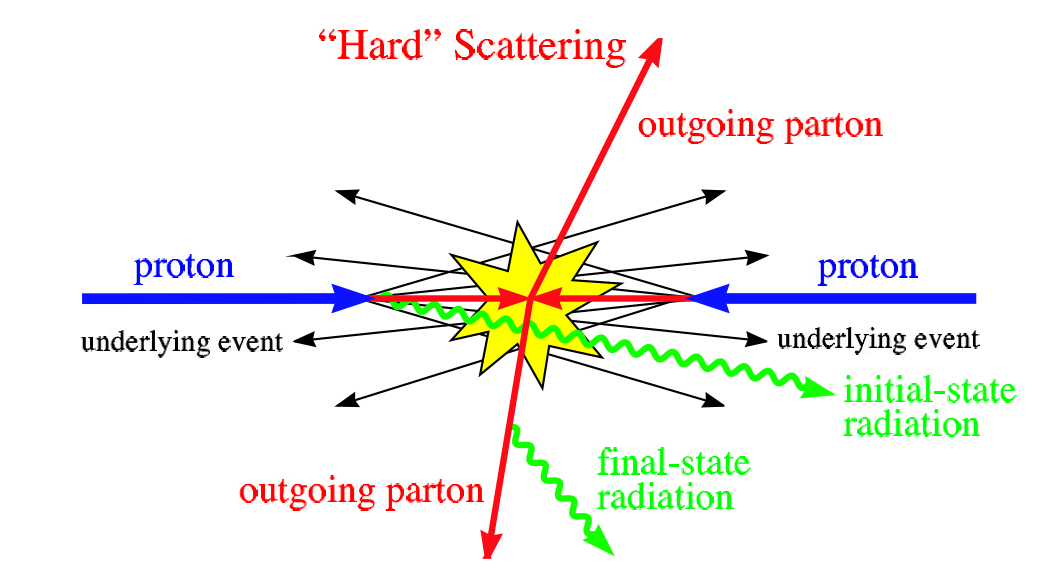
\includegraphics[width=0.7\textwidth]{Chapter2/HardProcess.png}
  \caption{Schematic representation of a hard scattering proton-proton
    collision. Figure from \cite{HardProcess}}
  \label{fig:HardProcess}
\end{figure}

Two incoming protons can be understood as the bag of
partons. The collision alone is dominated by the interaction of two partons - one from
each of the colliding hadrons. These partons are called incoming partons and the
momentum transfer by their interaction is $Q \gg \Lambda$, so the perturbative
QCD can be used in the process of hard scattering. Only a small fraction of
collision energy has remained for the rest of the partons, which create the so
called underlying event - particles, which do not come from
the dominant QCD processes.

The perturbative QCD is used, while the remnants from collision of incoming
partons are in distance $<10^{-15}\,\text{m}$ from each other. There is for
example enough time for top quark to decay. When the distance between outgoing
partons becomes greater, the non-perturbative QCD has to be used to describe the
hadronisation - the process, by which a set of colored partons is
transformed into a set of colorless primary hadrons which may then decay
further. 

During the collision, the electric and color charges of partons interact
resulting in radiation of photons $q \rightarrow q\gamma$ and gluons $q
\rightarrow qg$. These processes are described be perturbative QCD and lead to
infrared and collinear divergences. However, infrared divergences can be
canceled by Kinoshita--Lee--Nauenberg theorem \cite{KLN1,KLN2}, so only
collinear divergences remain. There is no mechanism known up to date, which
would solve the problem with collinear divergence. However, observables
inclusive enough to be insensitive to processes that distinguish between
different numbers of partons are not affected by infrared divergences.
There is no possibility how to theoretically predict the energy of hardest
outgoing particle, but it is possible to predict the energy flow in a cone from
the point of scattering.

This is where the term jet comes to play. A jet can be naively seen as a group
of collimated particles generated by the hadronisation of a parton in the
scattering process and is the most important object used on hadron colliders for
analysis of QCD processes.

\section{Jet Algorithms}

Jet algorithm is a generic "recipe" which takes a set of particles (or other
objects with defined
four-momenta) and returns jets created from them. That recipe usually involves a
set of parameters which together with the recipe fully specify the jet
definition. Following the remarks at the end of the previous section, jet
algorithms should fulfill following conditions 
\begin{enumerate}
  \item Infrared safety - the presence of additional soft particles between two
    particles belonging to the same jet should not affect the recombination of
    these particles into a jet.
  \item Collinear safety - jet reconstruction should not depend on fact, if
    transverse momentum is carried by one particle, or if a particle is split
    into two collinear particles.
\end{enumerate}

Principals of two jet algorithms are described here - fixed cone algorithm and
$k_t$ algorithm. First of these algorithms is more illustrative, the second one
is used in ATLAS. Detailed description as well as other jet algorithms can be
found in \cite{ATLASmain}. After definitions of jet algorithms it is shortly
described, how the objects (not necessary particles) with defined four-momenta
are constructed from the signal observed on the ATLAS detector.

\subsection{Fixed cone algorithm}

The first step of this algorithm is to order all input objects (reconstructed
detector objects with four-momentum representation) in decreasing order in
transverse momentum $\pt$. If the object with the highest $\pt$ is above the
seed threshold, all objects within a cone in pseudorapidity $\eta$ and azimuth
$\phi$ with $\Delta R = \sqrt{\Delta \eta^2 + \Delta \phi^2} < R_{cone}$, where
$R_{cone}$ is the fixed cone radius, are combined together. A new direction is
calculated from the four-momenta inside the initial cone and a new cone is
centered around it. Objects are then recollected in this new cone and again the
direction is updated. This process continues until the direction of the cone
does not change anymore after recombination, at which point the cone is
considered stable and is called a jet. At this point, the next seed is taken
from the input list and a new cone jet is formed with the same iterative
procedure. This continues until no more seeds are available. 

The jets found this way can share some constituents. This algorithm is both not
infrared safe (Figure \ref{fig:IRsafety}) and not collinear safe (Figure
\ref{fig:ColSafety}).

\begin{figure}[t]
  \centering
  \begin{subfigure}[b]{0.65\textwidth}
    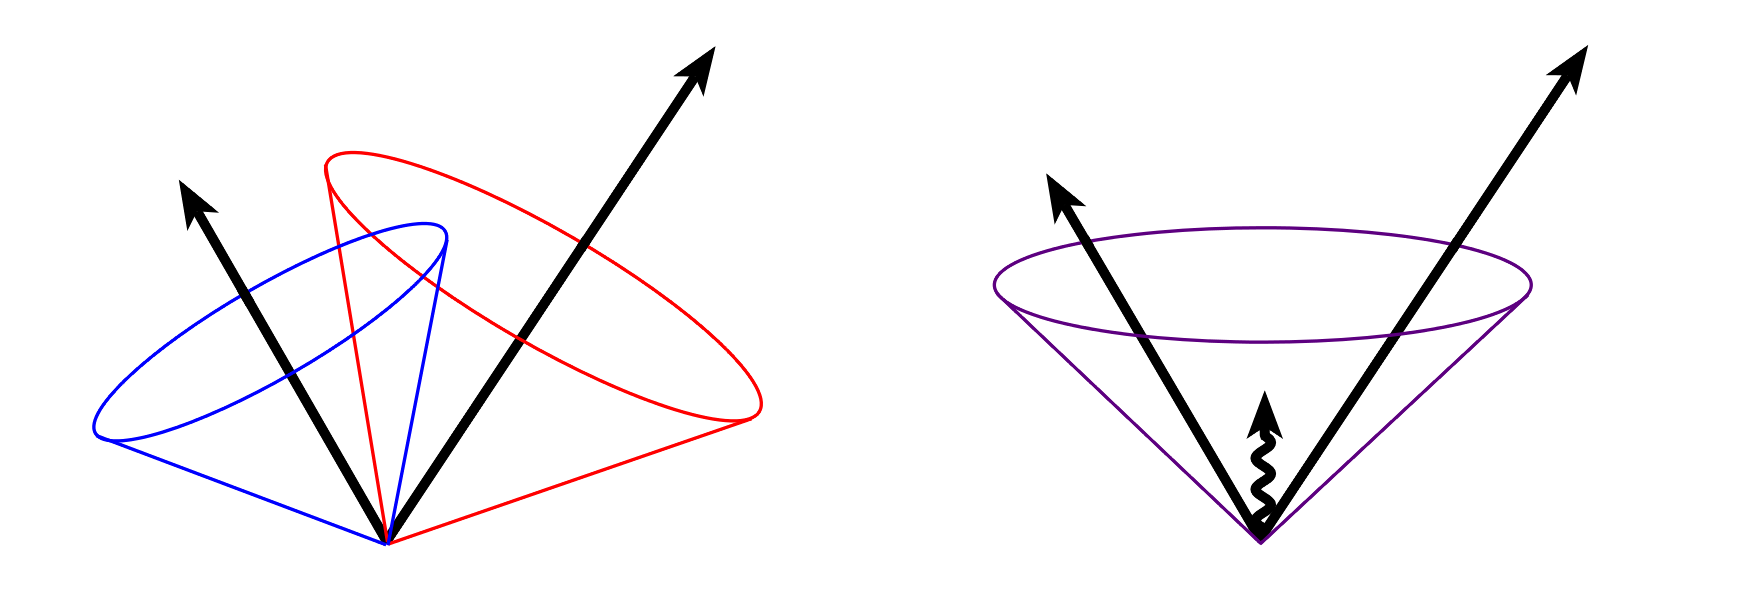
\includegraphics[width=\textwidth]{Chapter2/IRsafety.png}
    \caption{Infrared unsafety}
    \label{fig:IRsafety}
  \end{subfigure}
  ~
  \begin{subfigure}[b]{0.6\textwidth}
    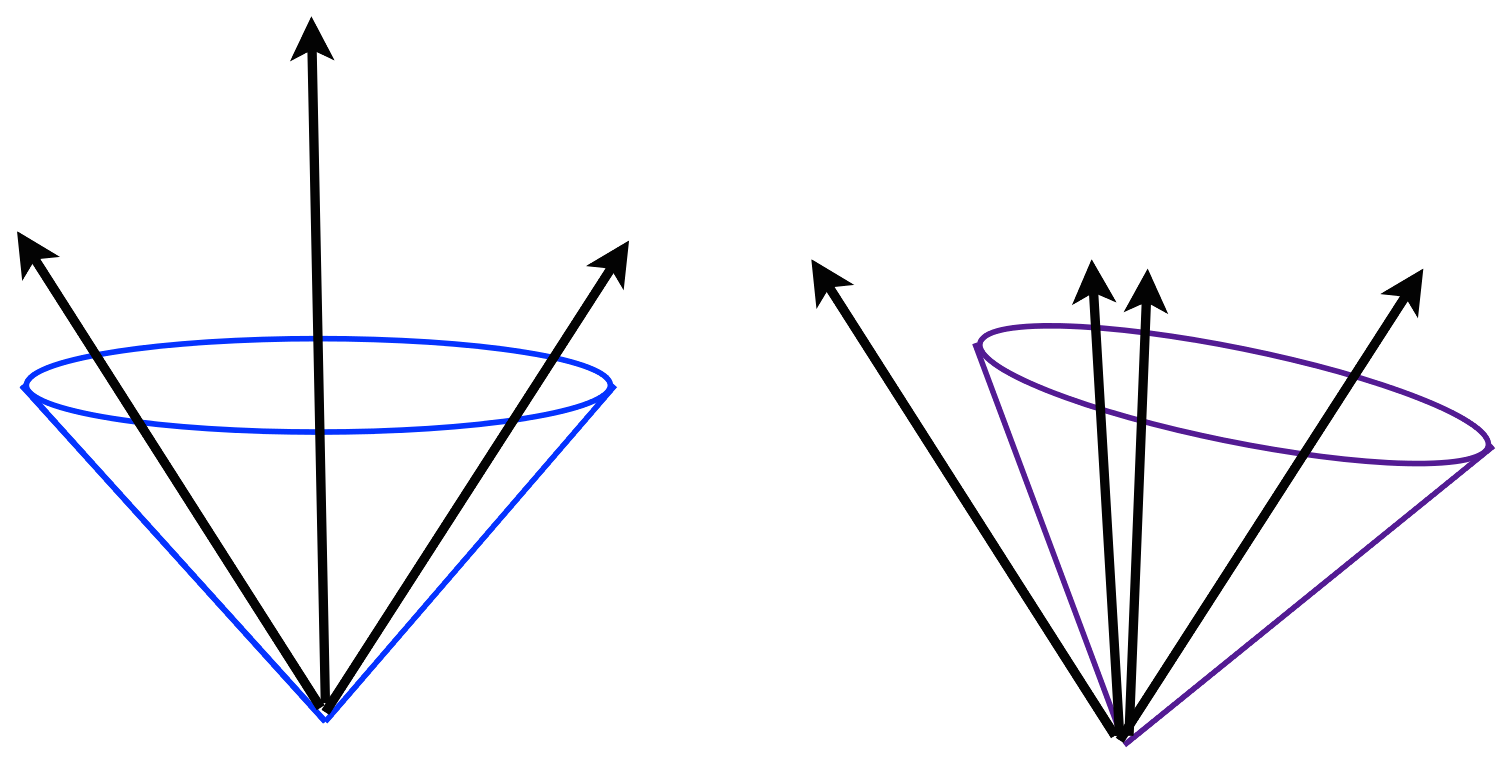
\includegraphics[width=\textwidth]{Chapter2/ColSafety.png}
    \caption{Collinear unsafety}
    \label{fig:ColSafety}
  \end{subfigure}
  \caption{Illustration of (a) infrared unsafety and (b) collinear unsafety
    of fixed cone jet algorithm.
    Figures from \cite{JetTheoreticalPictures}.}
  \label{fig:JetIRCOLsafety}
\end{figure}

Parameters used by fixed cone algorithm are a seed threshold of $\pt > 1 \GeV$,
and a narrow ($R_{cone} = 0.4$) or a wide cone jet ($R_{cone} = 0.7$) option.

\subsection{$k_t$ algorithms}

In this class of algorithms all pairs $(i,j)$ of input objects are analyzed with
respect to their relative transverse momentum squared, defined by 

\begin{equation}
	d_{ij} = \min{\left( p_{T,i}^{2p} , p_{T,j}^{2p} \right)} \frac{\Delta R_{ij}^2}{R^2}
\end{equation}
and the squared $\pt$ of object $i$ relative to the beam axis

\begin{equation}
	d_i = p_{T,i}^{2p}.
\end{equation}
Here $\Delta R_{ij}^2 = (y_i - y_j)^2 + (\phi_i - \phi_j)^2$ and $p_{T,i}$,
$y_i$ and $\phi_i$ are respectively the transverse momentum, rapidity and
azimuth of particle $i$. In addition to the radius parameter $R$, parameter $p$
was added to split $k_t$~algorithms into three categories.  
\begin{itemize}
	\item $p = 1$ $k_t$ algorithm,
	\item $p = 0$ Cambridge/Aachen algorithm,
	\item $p = -1$ anti-$k_t$ jet-clustering algorithm.
\end{itemize}
The differences between these algorithms are detailed described
in~\cite{ANTIKT}. Recombination of calorimeter signal towers (see Section
\ref{sse:CalorimeterJets}) in jets is for $k_t$ and anti-$k_t$ algorithms shown
at Figure 

\begin{figure}[t]
  \centering
  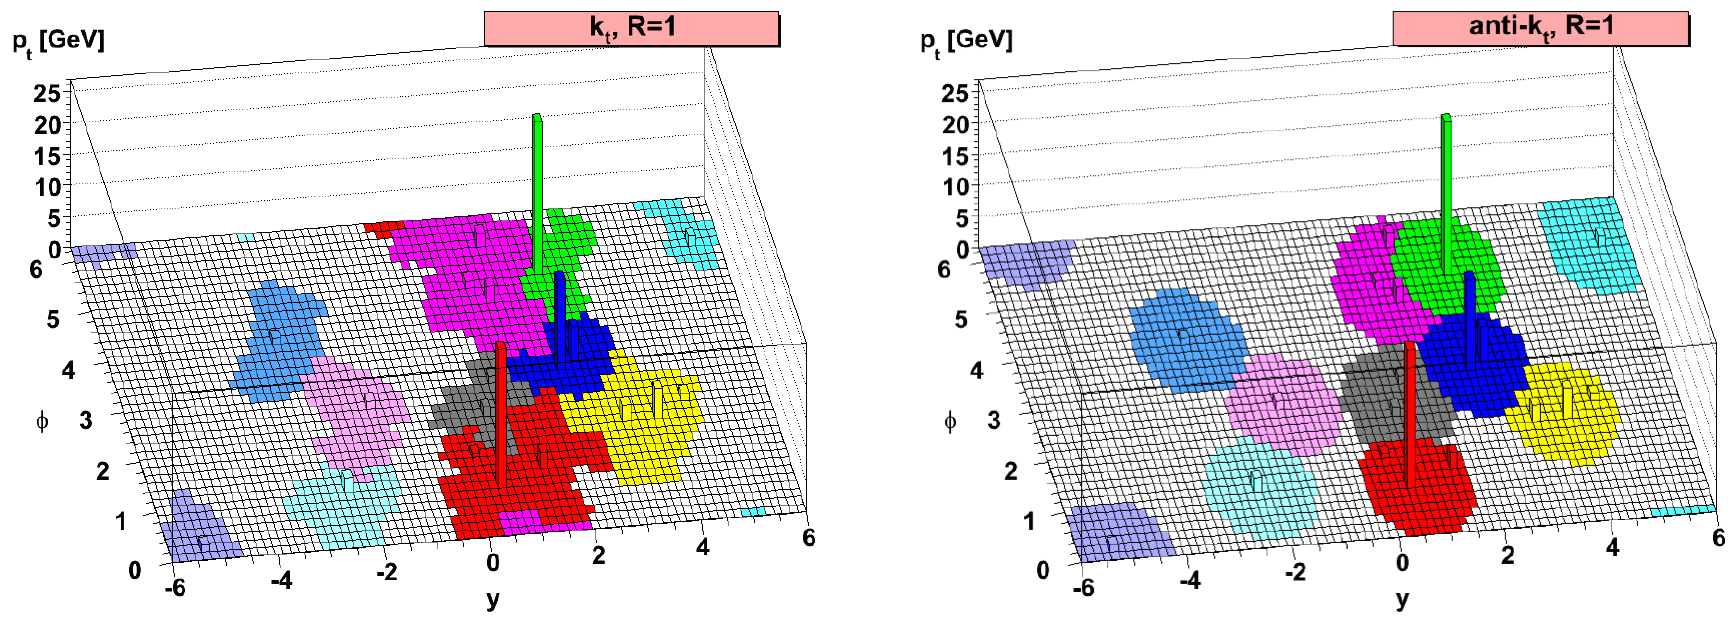
\includegraphics[width=\textwidth]{Chapter2/JetRecombination.png}
  \caption{Illustration of $k_t$ and anti-$k_t$ jet algorithms with $R=1$ for
    calorimeter signal towers in azimuth $\Phi$ and pseudorapidity $y$. Towers of
    the same color were recombined to one jet. Figure from
    \cite{JetTheoreticalPictures}} 
  \label{fig:JetRecombination}
\end{figure}

These algorithms first find the minimum $d_{min}$ of all $d_{ij}$ and $d_i$. If
$d_{min}$ is in $d_{ij}$'s, the corresponding objects $i$ and $j$ are combined
into a new object $k$ using four-momentum recombination. Both objects $i$ and
$j$ are removed from the list, and the new object $k$ is added to it. If
$d_{min}$ is in $d_i$'s, the object $i$ is considered to be a jet by itself and
removed from the list.

This means that all original input objects end up to be either part of a jet or
to be jets by themselves. Contrary to the cone algorithm described earlier, no
objects are shared between jets and the procedure is both infrared and collinear
safe.

ATLAS uses anti-$k_t$ algorithm with $R=0.4$ for narrow and $R=0.6$ for wide
jets.

\subsection{Calorimeter jets}
\label{sse:CalorimeterJets}

The most important detectors for jet reconstruction are the ATLAS calorimeters.
The ATLAS calorimeter system has about 200,000 individual cells of various sizes
and with different readout technologies and cell geometries. For jet finding it
is necessary to first combine these cell signals into larger signal object with
physically meaningful four-momenta. The two concepts available are calorimeter
signal towers and topological cell clusters.

In the case of calorimeter signal towers, the cells are projected onto a fixed
grid in pseudorapidity $\eta$ and azimuth $\phi$. The tower bin size is $\Delta
\eta \times \Delta \phi = 0.1 \times 0.1$ in the whole acceptance region of the
calorimeters, i.e. in $|\eta| < 5$ and $- \pi < \phi < \pi$ with approximately 
$100 \times 64 = 6,400$ towers in total.

The alternative representation of the calorimeter signals for jet
reconstruction are topological cell clusters, which are basically an attempt to
reconstruct three-dimensional "energy blobs" representing the showers developing
for each particle entering the calorimeter. The clustering starts with seed
cells with a signal-to-noise ratio, or signal significance $\Gamma = E_{cell} /
\sigma_{noise,cell}$, above a certain threshold $S$, i.e. $|\Gamma| > S = 4$.
All directly neighboring cells of these seed cells, in all three dimensions,
are collected into the cluster. Neighbors of neighbors are considered for
those added cells which have $\Gamma$ above a certain secondary threshold $N$
($|\Gamma| > N = 2$). Finally, a ring of guard cells with signal significances
above a basic threshold $|\Gamma| > P = 0$ is added to the cluster. After the
initial clusters are formed, they are analyzed for local signal maximums by a
splitting algorithm, and split between those maximums.

\section{Jet corrections}

Before jets can proceed to the data analysis, corrections have to be done to
minimize detector effects including calorimeter non-compensation, noise, losses
in dead material and cracks, longitudinal leakage and particle deflection in the
magnetic field. Indispensable tool for jet corrections are Monte Carlo event
generators - \textsc{Pythia} (?citace?) generating high-energy-physics events and 
\textsc{Geant4} (?citace?) or \textsc{AtlfastII} (?citace?) detector simulations
for simulating the detector response on \textsc{Pythia} generated events.

Using these tools it is possible to simulate jet reconstruction on three
different stages of collisions indicated in Figure \ref{fig:JetPhases}. First
there are parton jets which are reconstructed from the quarks, gluons and other
elementary particles created just after the collision. Stable particles (with
lifetime $c\tau \sim 10^{-15}\,\text{m}$) created by hadronization are recombined into
the particle jets. When collision reaches the detector, the detector simulation
is used and the recorded signal is reconstructed into signal jets.

\begin{SCfigure}
  \centering
  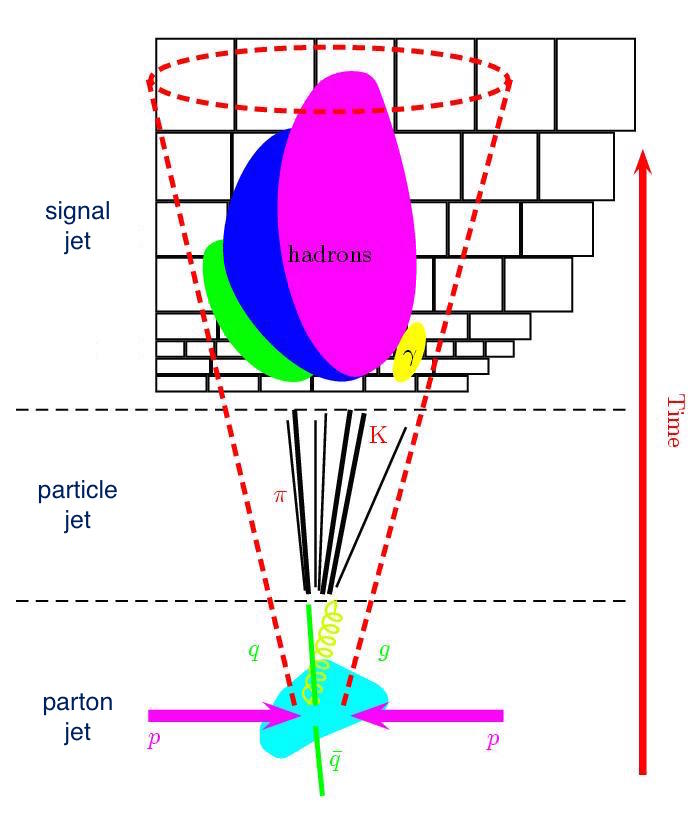
\includegraphics[width=0.6\textwidth]{Chapter2/JetPhases.jpg}
  \caption{Possible levels of jet reconstructions. Figure from \cite{DZero:JetEnergyScale} }
  \label{fig:JetPhases}
\end{SCfigure}

First the signal jets are corrected to the parton jets leading to modification
of kinematic properties of signal jets in the process called calibration.
Because the calibration is persistently evolving, each jet analysis uses as the
input the uncalibrated signal jets which are then easily calibrated using
standard library \textsc{ApplyJetCalibration} (?citace?).

There are some detector effects which are not removable by the calibration. These
effects include the limited detector resolution (detector cells have finite
dimensions) and the limited acceptance (not all events are recorded). The former
leads to the smearing of jet kinematic properties wheres the later to
lowering of observed cross section against the value theoretically
predicted. Both of these effects are negatively influencing the observables
and can be partially removed by the unfolding procedure, which unlike
the jet calibration, is analysis dependent. 

\subsection{Unfolding}

In this analysis, the distribution $f(\pt)$ of inclusive jet $\pt$ is measured
for $\pt \in \langle a, b \rangle$. Thanks to the detector imperfections,
instead of physical variable $\pt$ new variable $x$ and its distribution
$g(x)$ are measured. New distribution can be expressed as

\begin{equation}
  g(x) = \int_a^b A(x, \pt) f(\pt) dx,
  \label{eq:UnfoldingBasicDefinition}
\end{equation}
with the function $A(x, \pt)$ describing the detector response as can be seen
when the detector is exposed to a particle beam with well known $\pt = \pt'$
meaning $f(\pt) = \delta(\pt - \pt')$, leading to $g(x) = A(x, \pt')$. The
reconstruction of $f(\pt)$ from measured $g(x)$ is called unfolding.

For practical purposes the equation \eqref{eq:UnfoldingBasicDefinition} should
be discretized so instead of continuous distribution $g(x)$ the discretized
values $g_i = \int_{N(i)} g(x)dx$ of discretized observable $f_i =
\int_{N(i)} f(\pt)d\pt$ are measured, where the integral goes over measurable $N(i)
\subset \langle a, b \rangle$. For simplicity assume $x \in \langle
a, b \rangle$ is discretized in the same way as the physical $\pt$. Equation 
\eqref{eq:UnfoldingBasicDefinition} then reads

\begin{equation}
  g = Af,
  \label{eq:UnfoldingDiscretized}
\end{equation}
with $g$ and $f$ being vectors of $g_i$'s and $f_i$'s respectively and $A$ matrix
derived from $A(x, \pt)$. If the limited acceptance would be the only detector
problem, then $A$ would be diagonal matrix with some elements $ < 1$. When the
limited resolution comes to play, the diagonal entries starts to smear out of
the diagonal and the matrix $A$ starts to complicate.

The unfolding result which offers the solution of
\eqref{eq:UnfoldingDiscretized} by inversion of matrix $A$ is mostly
disappointing as is illustrated e.g. in (?citace?). For result improvement,
different unfolding methods were developed including iterative Bayesian
(?citace?), Singular Value Decomposition (?citace?), or iterative, dynamically
stabilized (IDS) method (?citace?), which is the method used in this thesis. 


